\documentclass{article}

% Language setting
% Replace `english' with e.g. `spanish' to change the document language
\usepackage[english]{babel}
\usepackage{tabularx}
\usepackage{subfigure}
\usepackage{amsmath}

% Set page size and margins
% Replace `letterpaper' with `a4paper' for UK/EU standard size
\usepackage[letterpaper,top=2cm,bottom=2cm,left=3cm,right=3cm,marginparwidth=1.75cm]{geometry}

% Useful packages
\usepackage{amsmath}
\usepackage{graphicx}
\usepackage[colorlinks=true, allcolors=blue]{hyperref}

\title{Control Policy Design for Path Planning and Obstacle Avoidance Using Optimal Trajectory Generation of a Four-Wheel Based Extraterrestrial Rover}
\author{Jason Zhou\{zzhou292@wisc.edu\}, Yulong Yue\{yyue32@wisc.edu\}}

\begin{document}
\maketitle


\section{Research Problem Statement}
In this project, we proposed to design a rover path planning and following algorithm to provide an extraterrestrial rover navigation strategy. We propose to solve the problem by solving a closed-loop motion planning and control problem based on optimization with constraints. The control strategy will be benched in a simulated environment in Project Chrono. For the project, we will assume privileged information, such as locations, sizes, and shapes of the obstacles. Also, we will assume the environment is limited and fixed. 


\section{Background}
\subsection{Rover Control Strategy}
Providing control solutions to extraterrestrial rover can always be challenging, due to the low tolerance to mistake and long signal transmission delay. Nowadays, most space exploration agencies, such as The National Aeronautics and Space Administration (NASA), are adopting two different ways for rover control:

\begin{itemize}
    \item Manual Explicit Motion Commands
    \item A propitiatory Autonomous Path Planning and Path Following Control Policies
\end{itemize}

The first manual control strategy is relatively simple. Based on the images transmitted from the rover, the ground base provides direct motion commands, such as "move forward for 5m", to the rover. The method relies heavily on human judgment, along with data and command transmission, which usually suffer from the signal delay between the ground base on earth and extra extraterrestrial planets. This control method will not be discussed in the project.

The second control method, although proprietary and few details have been disclosed by NASA, is an autonomous path planning and trajectory following control algorithm which matches the materials covered in the class. Based on the introduction provided by NASA, the ground base on earth, based on the images and data transmitted from the rover, sends a control signal containing the location of the next 'waypoint'. Then the rover, based on its own sensing capabilities using sensors such as camera and lidar, plans the route and tracking the planned trajectory. \cite{NASAweb}

\subsection{Simulation Through Project Chrono}
\label{subsec:chrono}
Project Chrono is a multi-physics modeling and simulation infrastructure based on a platform-independent, open-source design. Project Chrono has been used widely for the simulation of autonomous vehicles and robotic systems. Project Chrono, in the past two years, received funding from NASA to provide simulation support to investigate wheel-terrain interaction of the 2024 NASA VIPER Moon Rover using different types of terra-mechanics simulation method, as shown in Figure \ref{fig:viper_chrono} and Figure \ref{fig:curiosity_chrono}. Therefore, the software package already contains multiple ready-to-deploy extraterrestrial rover models and their control interfaces. 

In this project, we will develop the algorithm in Matlab, and use Project Chrono as our simulation environment. In the simulation, we will use the Soil-Contact Model (SCM) deformable terrain model to simulation soil deformation. The SCM model is a simple semi-empirical model which is built upon the original Bekker-Wong Equation, as shown in Equation \ref{equ:bekker}. A more detailed description can be found in \cite{10.1115/1.4056851}. In the Equation \ref{equ:bekker}, \(K_{c}\), \(K_{\phi}\), and n are semi-empirical parameters defining the soil properties, \(z\) is the sinkage, \(b\) is the average wheel contact width, and \(p\) is the normal pressure applied to the rover wheel (to provide normal force in the simulation).

\begin{equation}\label{equ:bekker}
	p = \left( \frac{K_c}{b} + K_\phi \right) z^n \, .
\end{equation}

\begin{figure}
	\centering     %%% not \center
	\subfigure[Curiosiy Mars rover on SCM deformable terrain with lidar and radar sensing simulation]{
		\label{fig:curiosity_chrono}
		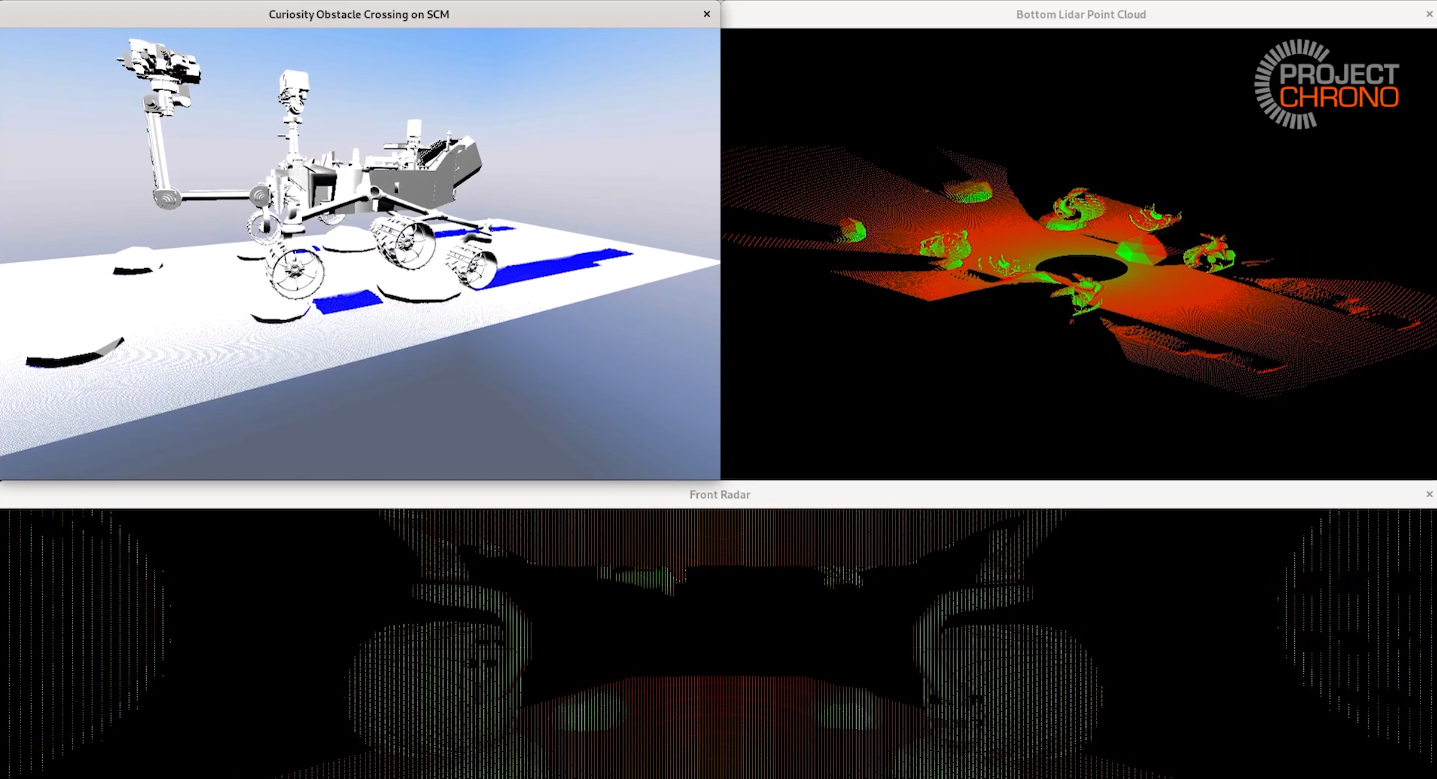
\includegraphics[width=0.45\textwidth]{Images/Curiosity_Sensing.png}}
	\subfigure[VIPER Lunar rover conducting bulldozing experiment on granular terrain simulated by Smoothed-Particle Hydrodynamics (SPH) Method]{
		\label{fig:viper_chrono}
		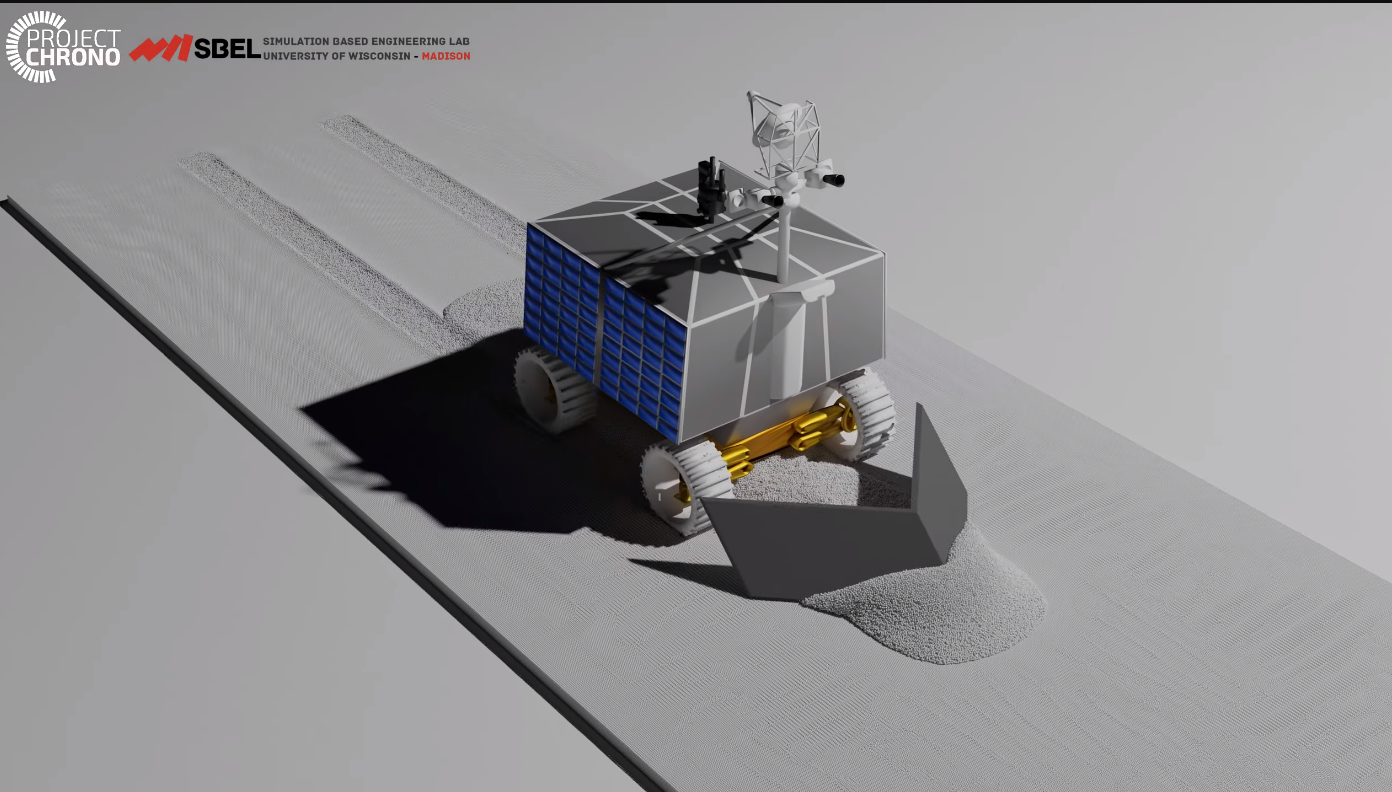
\includegraphics[width=0.45\textwidth]{Images/Viper_Bull.png}}
	\caption{Project Chrono contains complete rover models, control interfaces, and deformable terrain models for wheel-terrain interaction}
\end{figure}


\section{Proposed Solution}

The problem is dissected into two parts - trajectory generation and trajectory tracking in simulation. The first part, trajectory generation, is conducted using Imperial College London Optimal Control Software (ICLOCS 2), An Optimization Based Control package in Matlab/Simulink. The optimization trajectory generation problem simplifies the problem by reducing it to 2-D and employing simplified rover dynamics, while representing obstacles as bounding circles. After trajectory has been generated, the planned path is parsed into a .csv file consisting of 200 way points. 

In the second stage, known as trajectory tracking in simulation, the Project Chrono platform is utilized. The rover's complete dynamics, encompassing various components such as the DC motors, chassis, steering mechanism, and suspension system, are accurately modeled. The simulation is structured as a multi-body dynamic problem that incorporates rigid bodies and constraints between different bodies. The terrain is simulated through a semi-empirical deformable model called the Soil-Contact Model (SCM), which is explained in detail in Section \ref{subsec:chrono}. The output trajectory obtained from the previous stage is then reconstructed into a Bézier curve, which the rover aims to pursue in the simulation. For the current problem, a PID controller is used for trajectory tracking.

\subsection{Trajectory Generation}

The problem is simplified into an optimal path planning and control optimization problem by assuming a square terrain with a center at (0.0, 0.0), and a fixed side length of 20 meters. Three different types of rocks with similar radius, while viewing birdeye view, are used. To further simplify the problem, a bounding circle, or what can be called a safety circle, is drawn around the rock. From a bird's eye view, looking from above, the problem environment is simplified into a 2D path planning and optimal control problem with a given square terrain, and with several circular-shaped obstacles, as shown in Figure \ref{fig:rover_path}.

We employ a dynamic model of a simplified rover as shown in Equations \ref{equ:car_dyn}.

\begin{equation}
\label{equ:car_dyn}
  \left\{\begin{array}{@{}l@{}}
    \dot{x}=v(t)cos(\theta(t))  \\
    \dot{y}=v(t)sin(\theta(t))  \\
    \dot{v}(t) = a(t) \\
    \dot{a}(t) = u_{1}(t) \\
    \dot{\theta}(t) = \frac{v(t)tan(\phi(t))}{l_{a}} \\
    \dot{\phi}=u_{2}(t) \\
  \end{array}\right.\,.
\end{equation}

After the simplification, we assume that each obstacle has the properties shown in Equation \ref{equ:car_cons}, in which \(x_{obs_{k}}\) and \(y_{obs_{k}}\) represent the location of the k'th obstacle's bounding circle, and \(r_{obs_{k}}\) represent the radius of the bounding circle of the k'th obstacle. If we assume the entire time domain of the problem is $t_{f}$, and there are M obstacles presented in the environment. Assuming the starting location of the rover is \([\) \(x_{start}\), \(y_{start}\) \(]\), the given target location is \([\) \(x_{end}\), \(y_{end}\) \(]\), the initial rover yaw angle is $yaw_{t_{0}}$, and the initial rover steering angle $0$. We formulate the initial condition, terminal condition, and path constraint for the optimal control problem: 

\begin{equation}
	\label{equ:car_cons}
	\left\{\begin{array}{@{}l@{}}
		x(0) = x_{start}, y(0) = y_{start}  \\
		x(t_{f}) = x_{end}, y(t_{f}) = y_{end}  \\
		\theta(0) =yaw_{t_{0}}  \\
		\phi(0) = 0 \\
		r(k) < (x(t)-x_{obs_{k}})^2 + (y(t)-y_{obs_{k}})^2  \\
		0 \leq t \leq t_{f}, 0 \leq k \leq M \\
	\end{array}\right.\,.
\end{equation}

In addition to the above path constraints, the vehicle dynamic and state constraints are formulated as below:

\begin{equation}
	\label{equ:car_dyn_con}
	\left\{\begin{array}{@{}l@{}}
		-10 \leq x(t) \leq 10, -10 \leq y(t) \leq 10  \\
		 0 \leq v(t) \leq 3.0 \\
		 0 \leq a(t) \leq 0.8 \\
		 -\frac{\pi}{6} \leq \phi \leq \frac{\pi}{6} \\
	\end{array}\right.\,.
\end{equation}

Where the position states, $x(t)$ and $y(t)$, are bounded between -10 and 10, the square terrain which we pre-defined. The magnitude of the velocity of the rover is bounded between 0.0 $m/s$ and 3.0 $m/s$, and the magnitude of the acceleration of the rover is bounded between 0.0 $\frac{m}{s^2}$ and 0.8 $\frac{m}{s^2}$. Note that the constraints for the velocity magnitude and acceleration magnitude implies that the path generated from the optimization problem considers forward movement only, and no reverse motion is considered. The max steering, $\phi$, is bounded between -30 $deg$ to 30 $deg$, or $-\frac{\pi}{6}$ and $\frac{\pi}{6}$.  

An extra constraint is added to ensure on-board equipment's stability:

\begin{equation}
	\label{equ:car_stability}
	-0.4 \leq \frac{u_{2}(t)}{l_{axes}cos^{2}(\theta(t) )} \leq 0.4 \\
\end{equation}

In the above equation, the $l_{axes}$ represents the distance between two axes of the rover. For the Viper lunar rover which is modeled in this project, the $l_{axes} = 1.4 m$. In addition to the above constrains defined, a maximum final time is defined, as below:

\begin{equation}
	\label{equ:time_cons}
	0 \leq t_{f} \leq 100 \\
\end{equation}

The objective is for rover to finish the path in minimum time, as a results, the optimal control problem is formulated as:

\begin{equation}
	\label{equ:car_opt}
	\min_{x,u,t_{f}}t_{f}\\
\end{equation}


\begin{figure}
\centering
    \label{fig:rover_path}
    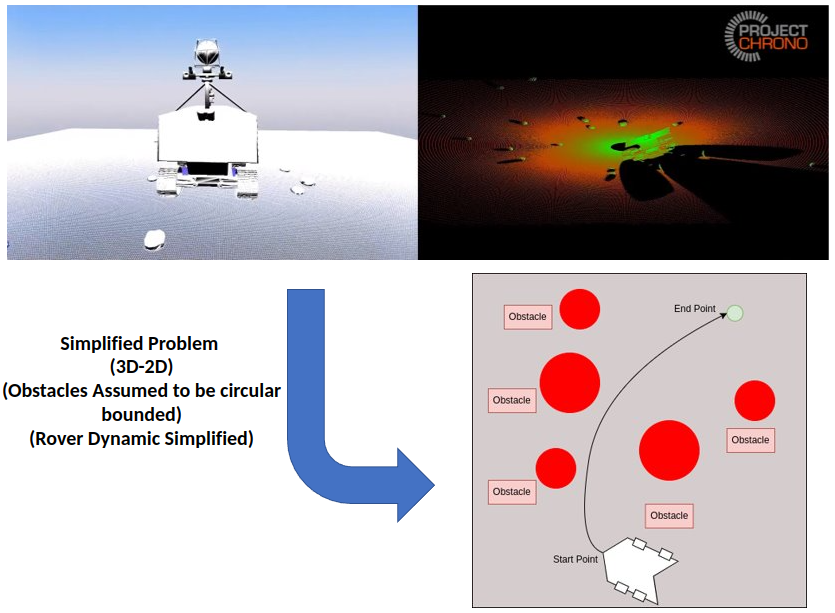
\includegraphics[width=0.85\textwidth]{Images/rover_path.png}
    \caption{The problem will be simplified into a 2-dimensional path planning and optimal control problem. The optimization will be solved in the 2-D space and applied and benched in the 3-D simulation.}
\end{figure}

\subsection{Trajectory Tracking in Simulation}

After the optimization problem has been solved, a control input series \(u_{opt}\) and a control path series defined by \(x_{opt}\) and \(y{opt}\) are expected to be the output. However, the control input series \(u_{opt}\) will need to be post-processed in order to feed into the Chrono simulation. This is due to the fact that the simplified rover dynamic equations defined in Equation \ref{equ:car_dyn} is a significantly simplified control, and the environment and the obstacle modeling are simplified as well. However, the actual rover control and rover dynamic response, using a high-fidelity rover dynamic modeling and simulation, depend on multiple factors, such as wheel-terrain interaction, DC motor modeling, steering and suspension mechanisms and etc. 

Therefore, only the optimal path obtained from the first part, trajectory generation, is used, and the second part of the problem is formulated as trajectory tracking. The path obtained from the trajectory generation consists of 200 way points, which are reconstructed into a Bézier curve for easier evaluation and tracking. A simple PID controller is used for tracking, as shown below:

\begin{equation}
	\label{equ:pid_ctr}
	u(t) = K_{p}e(t) + K{i}\int_{0}^{t}e(\tau)d\tau+K_{d}\frac{de(t)}{dt}
\end{equation}

The error term $e(t)$, in Equation \ref{equ:pid_ctr}, is defined as below: 

\begin{equation}
	\label{equ:pid_err}
	\left\{\begin{array}{@{}l@{}}
	s(t) = A_{local}^{global}(t)(m_{dist}*[1.0, 0.0, 0.0]^{T})  \\
	t(t) = eval(s(t)) \\
	\hat{y}(t) = A_{local}^{global}(t)([0.0, 1.0, 0.0]^{T})  \\
	e(t) = (s(t)-t(t))*(\hat{y}(t)) \\ 
	e(t) = clamp(e(t),-1.0, 1.0)  \\
	\end{array}\right.\,.
\end{equation}


Equation \ref{equ:pid_err} involves several variables. Firstly, $m_{dist}$ denotes the lookahead distance, while $s(t)$ represents the sentinel point. Secondly, $t(t)$ refers to the target point on the Bézier curve that is in proximity to the sentinel point $s(t)$. Lastly, $\hat{y}(t)$ is a unit vector oriented towards the rover's lateral direction. Notably, the error term $e(t)$ is limited between -1 and 1, signifying the maximum left and right steering errors, respectively. Note that since in the current problem setup, the rover is moving relatively slow using a linear DC motor model with maximum rotational speed $\pi$ $rad/s$ and a stall torque of 300 $N/m$. By conducting serval experiments, it is believed that a positive K value is good enough for trajectory tracking to work relatively well.

\section{Results}
4 different obstacle arrangement has been tested and examined, the positions of the obstacles, and the scenario parameters for each testing case are shown in Table \ref{tab:sce_setup} and Table \ref{tab:sce_obs}. Note that 3 rock geometries are used and they have similar geometry. Therefore, for simplification, a 1.5-m radius is used for all obstacle geometries.

\begin{table}[]
	\centering
	\begin{tabular}{|c|c|c|c|}
		\hline
		& \textbf{Initial Rover Position} & \textbf{Initial Rover Yaw Angle} & \textbf{Final Rover Position} \\ \hline
		\textbf{Scenario 1} & {[}-5.0, -6.0{]}                & 60 deg                           & {[}0.0, 8.0{]}                \\ \hline
		\textbf{Scenario 2} & {[}-6.0, -7.0{]}                & 110 deg                          & {[}8.0, 4.8{]}                \\ \hline
		\textbf{Scenario 3} & {[}-6.0, -7.0{]}                & 110 deg                          & {[}0.0, 8.0{]}                \\ \hline
		\textbf{Scenario 4} & {[}-5.0, 4.0{]}                 & 30 deg                           & {[}9.0, -8.0{]}               \\ \hline
	\end{tabular}
	\caption{Rover's initial position, final position, and initial yaw angle for each scenario.}
	\label{tab:sce_setup}
\end{table}

\begin{table}[]
	\centering
	\begin{tabular}{|c|l|l|l|l|l|}
		\hline
		& \multicolumn{1}{c|}{\textbf{Obs 1}}  & \multicolumn{1}{c|}{\textbf{Obs 2}}   & \multicolumn{1}{c|}{\textbf{Obs 3}}  & \textbf{Obs 4}  & \textbf{Obs 5}   \\ \hline
		\textbf{Scenario 1}             & \multicolumn{1}{c|}{{[}2.0, 0.0{]}}  & \multicolumn{1}{c|}{{[}-4.0, -1.0{]}} & \multicolumn{1}{c|}{{[}0.0, 1.2{]}}  & {[}3.0, 5.0{]}  & {[}-3.0, 2.0{]}  \\ \hline
		\textbf{Scenario 2}             & \multicolumn{1}{c|}{{[}3.0, -2.0{]}} & \multicolumn{1}{c|}{{[}-3.0, 1.0{]}}  & \multicolumn{1}{c|}{{[}0.0, -0.2{]}} & {[}8.0, -2.5{]} & {[}-3.0, -2.0{]} \\ \hline
		\textbf{Scenario 3}             & \multicolumn{1}{c|}{{[}5.0, -1.4{]}} & \multicolumn{1}{c|}{{[}0.2, 4.8{]}}   & \multicolumn{1}{c|}{{[}0.0, 0.0{]}}  & {[}6.4, 4.5{]}  & {[}-3.8, -2.0{]} \\ \hline
		\textbf{Scenario 4}             & \multicolumn{1}{c|}{{[}3.0, -3.4{]}} & \multicolumn{1}{c|}{{[}-5.2, -7.8{]}} & \multicolumn{1}{c|}{{[}0.0, 0.8{]}}  & {[}7.4, -1.3{]} & {[}-6.8, 2.0{]}  \\ \hline
		\multicolumn{1}{|l|}{\textbf{}} & \textbf{Obs 6}                       & \textbf{Obs 7}                        & \textbf{Obs 8}                       & \textbf{Obs 9}  & \textbf{Obs 10}  \\ \hline
		\textbf{Scenario 1}             & {[}7.0, 1.0{]}                       & {[}4.0, -7.0{]}                       & {[}-8.0, 5.0{]}                      & {[}7.6, -4.0{]} & {[}-8.1, -2.3{]} \\ \hline
		\textbf{Scenario 2}             & {[}5.0, 3.0{]}                       & {[}3.2, 4.0{]}                        & {[}-8.0, 7.0{]}                      & {[}5.8, 6.7{]}  & {[}-7.2, -2.3{]} \\ \hline
		\textbf{Scenario 3}             & {[}3.5, 3.0{]}                       & {[}-2.8, 4.0{]}                       & {[}-8.0, 8.0{]}                      & {[}2.8, -3.7{]} & {[}-7.2, 2.3{]}  \\ \hline
		\textbf{Scenario 4}             & {[}1.9, -7.1{]}                      & {[}6.8, 4.0{]}                        & {[}6.9, 7.0{]}                       & {[}-3.8, 0.0{]} & {[}-7.2, 6.3{]}  \\ \hline
	\end{tabular}
	\caption{Obstacle setup for each scenario. }
	\label{tab:sce_obs}
\end{table}


\begin{figure}
	\centering     %%% not \center
	\subfigure[Scenario 1]{
		\label{fig:traj_1}
		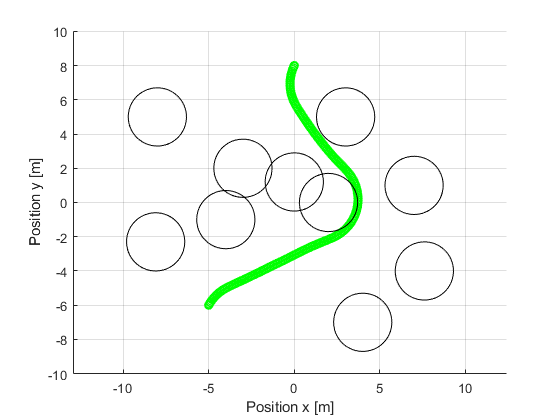
\includegraphics[width=0.45\textwidth]{Images/iclocs/traj_1.png}}
	\subfigure[Scenario 2]{
		\label{fig:traj_2}
		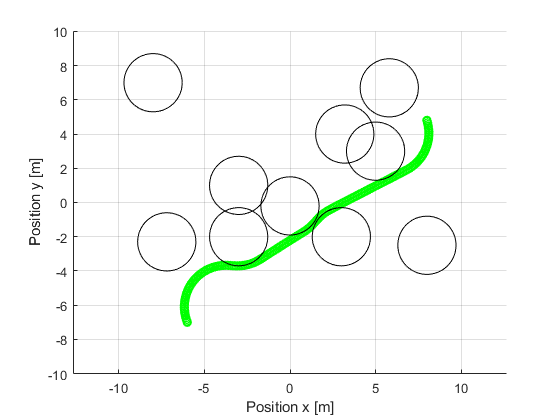
\includegraphics[width=0.45\textwidth]{Images/iclocs/traj_2.png}}
	\subfigure[Scenario 3]{
		\label{fig:traj_3}
		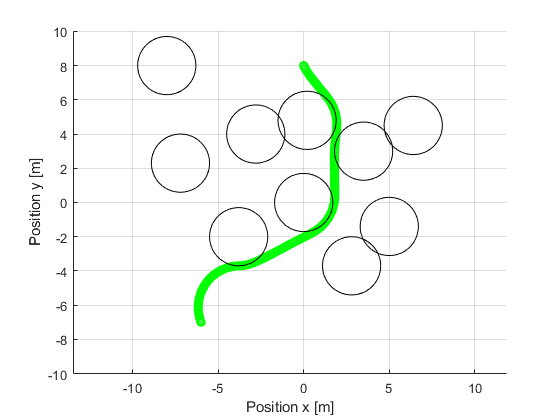
\includegraphics[width=0.45\textwidth]{Images/iclocs/traj_3.png}}
	\subfigure[Scenario 4]{
		\label{fig:traj_4}
		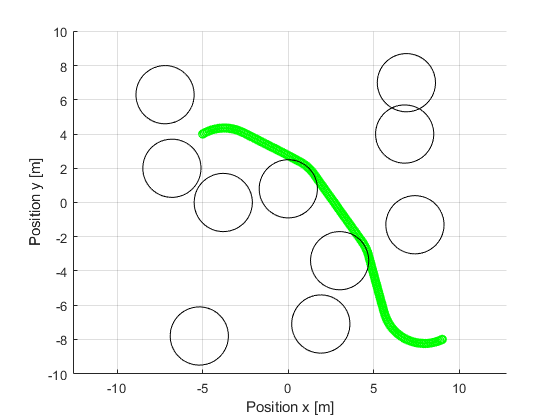
\includegraphics[width=0.45\textwidth]{Images/iclocs/traj_4.png}}
	
	\caption{Trajectories generated by ICLOCS. In the each figure, the green curve is the optimal trajectory and each circle represents the bounding circle of each obstacle. }
\end{figure}


\begin{figure}
	\centering     %%% not \center
	\subfigure[Scenario 1 \cite{sce-1}]{
		\label{fig:screen_1}
		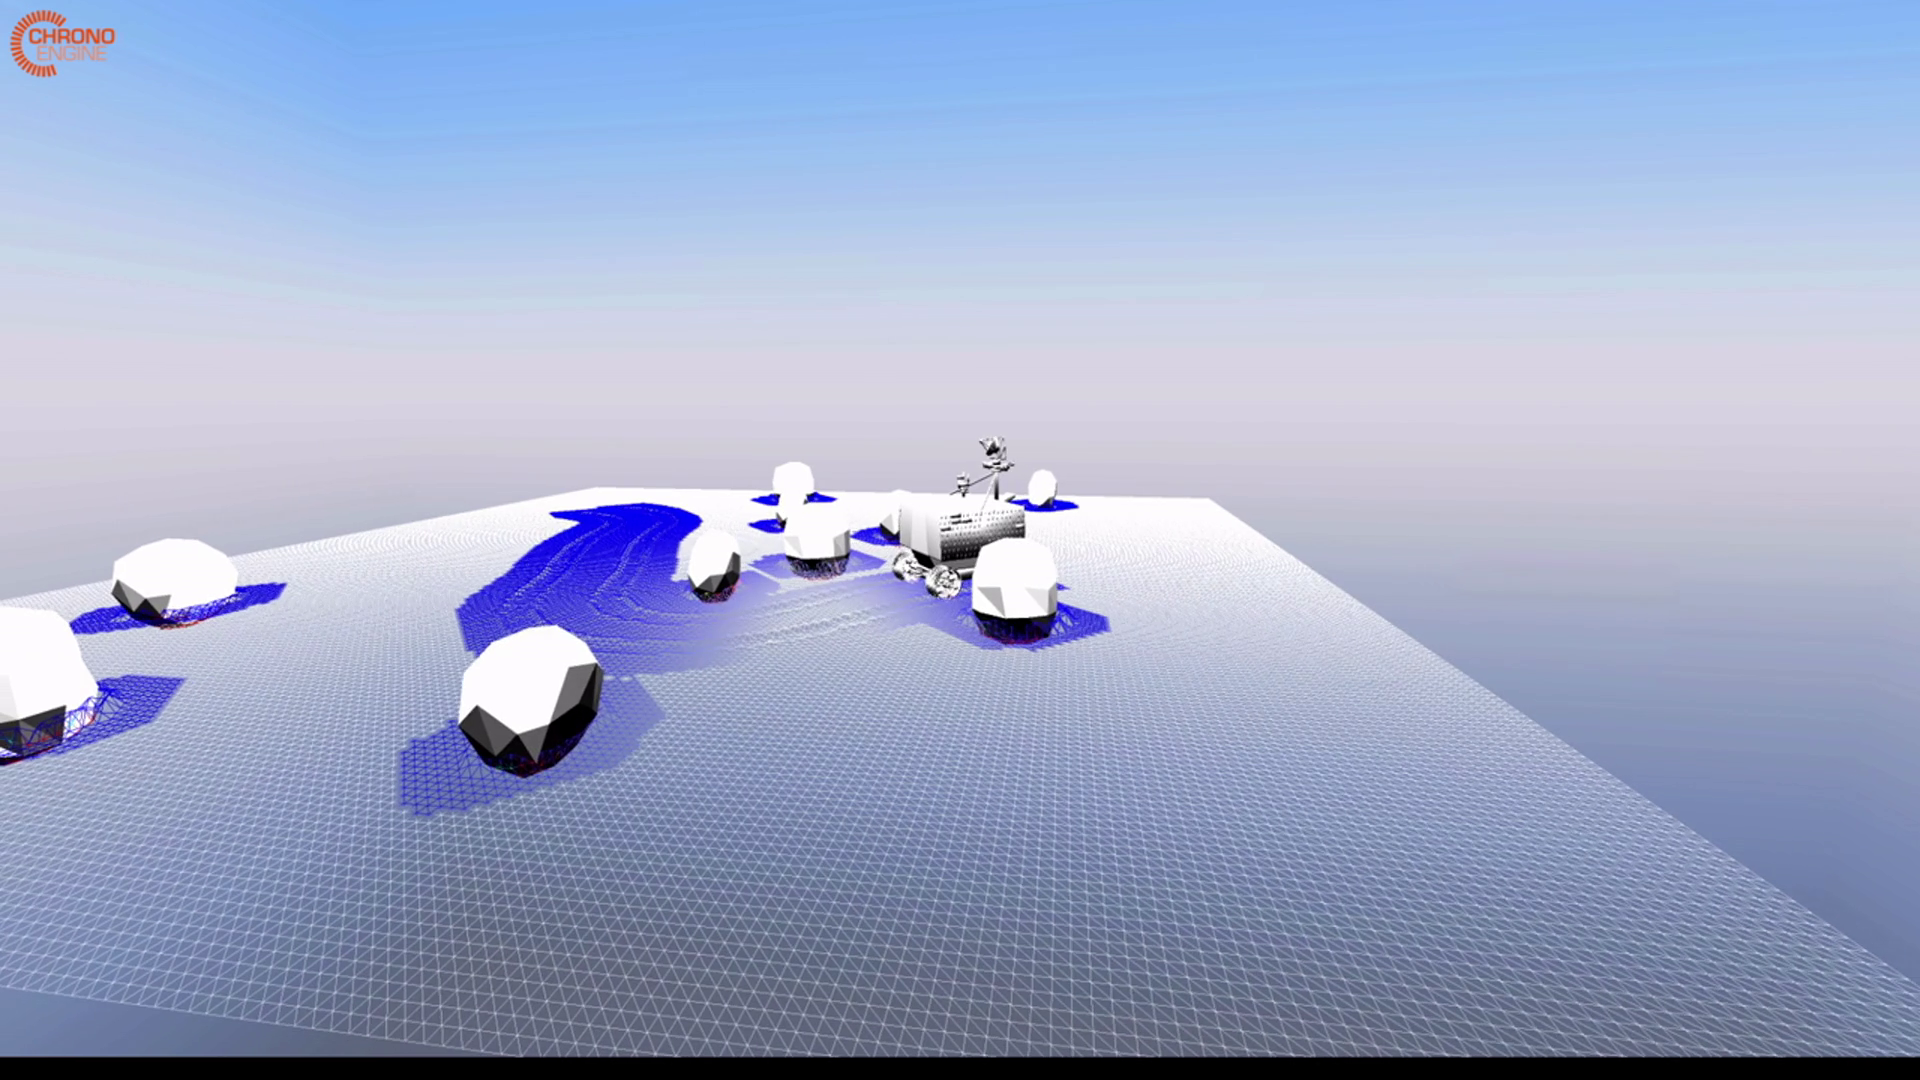
\includegraphics[width=0.45\textwidth]{Images/screenshot/1.png}}
	\subfigure[Scenario 2 \cite{sce-2}]{
		\label{fig:screen_2}
		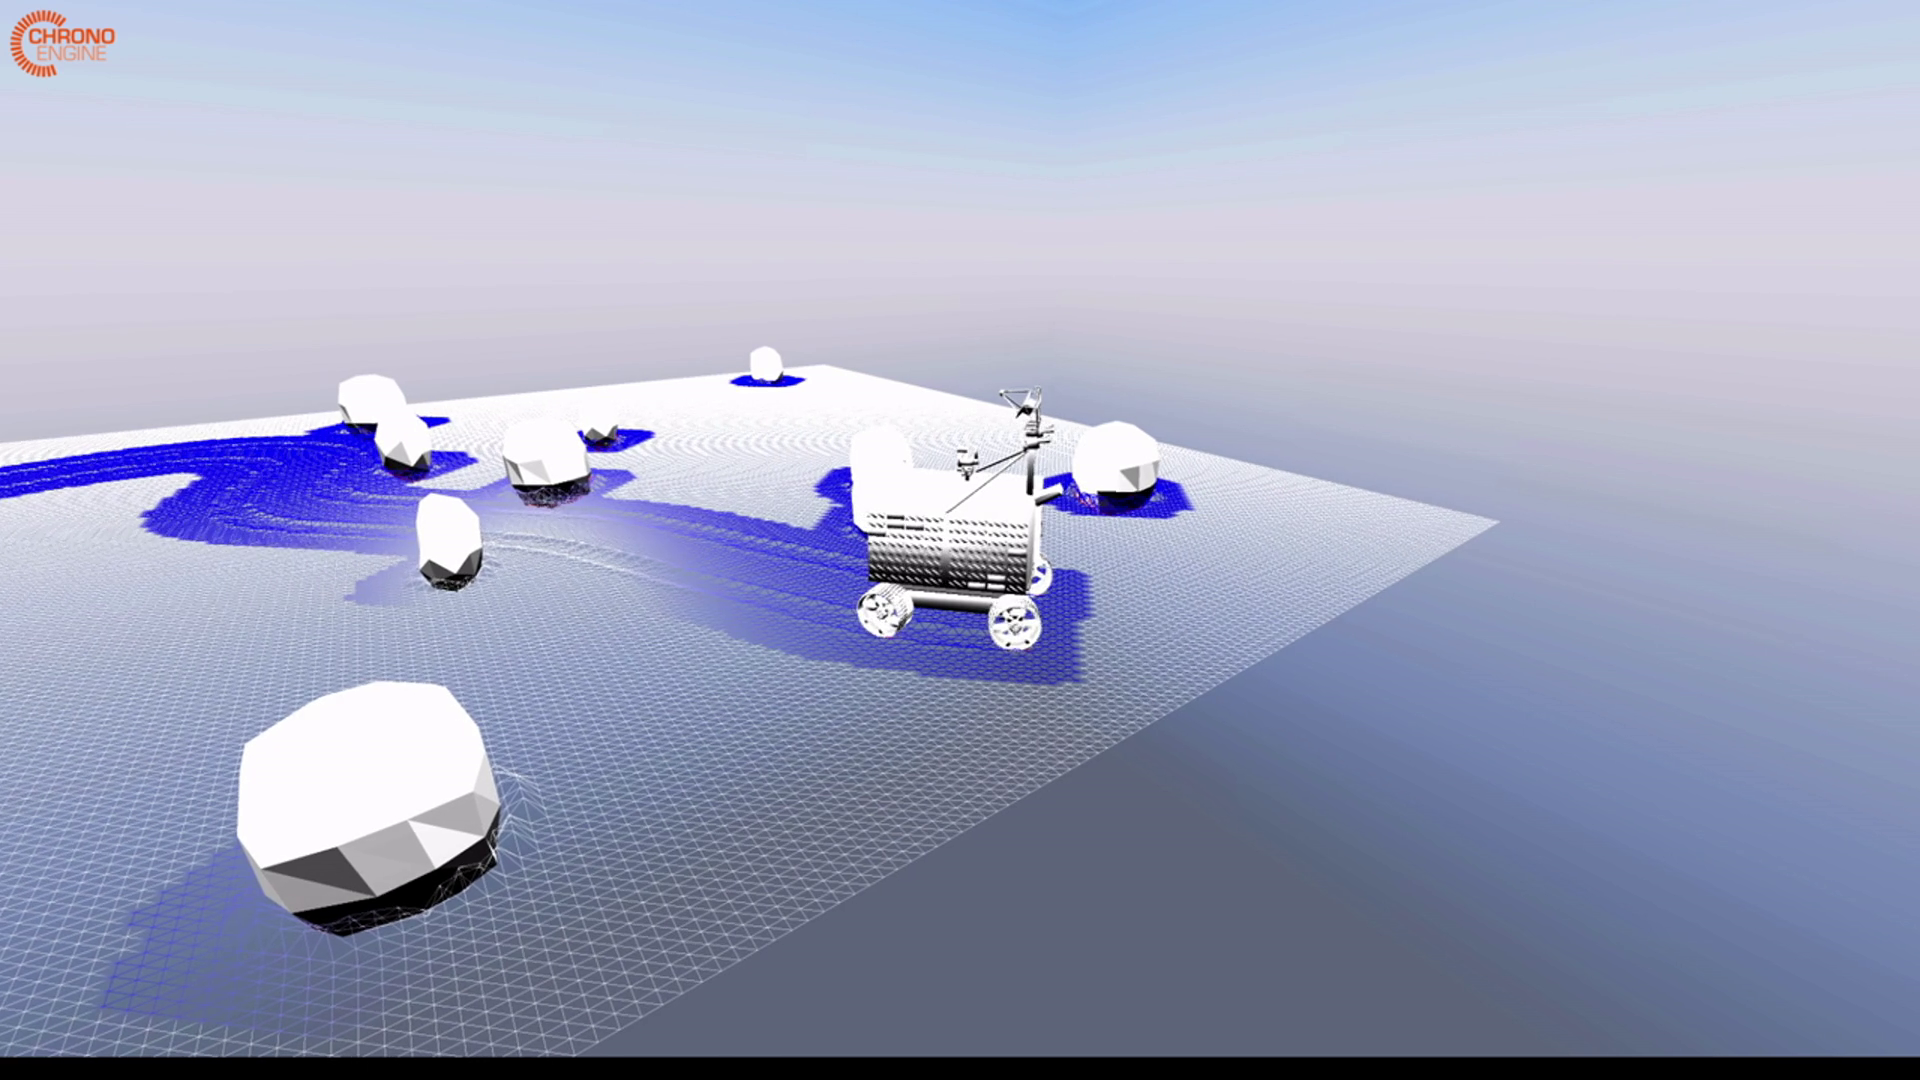
\includegraphics[width=0.45\textwidth]{Images/screenshot/2.png}}
	\subfigure[Scenario 3 \cite{sce-3}]{
		\label{fig:screen_3}
		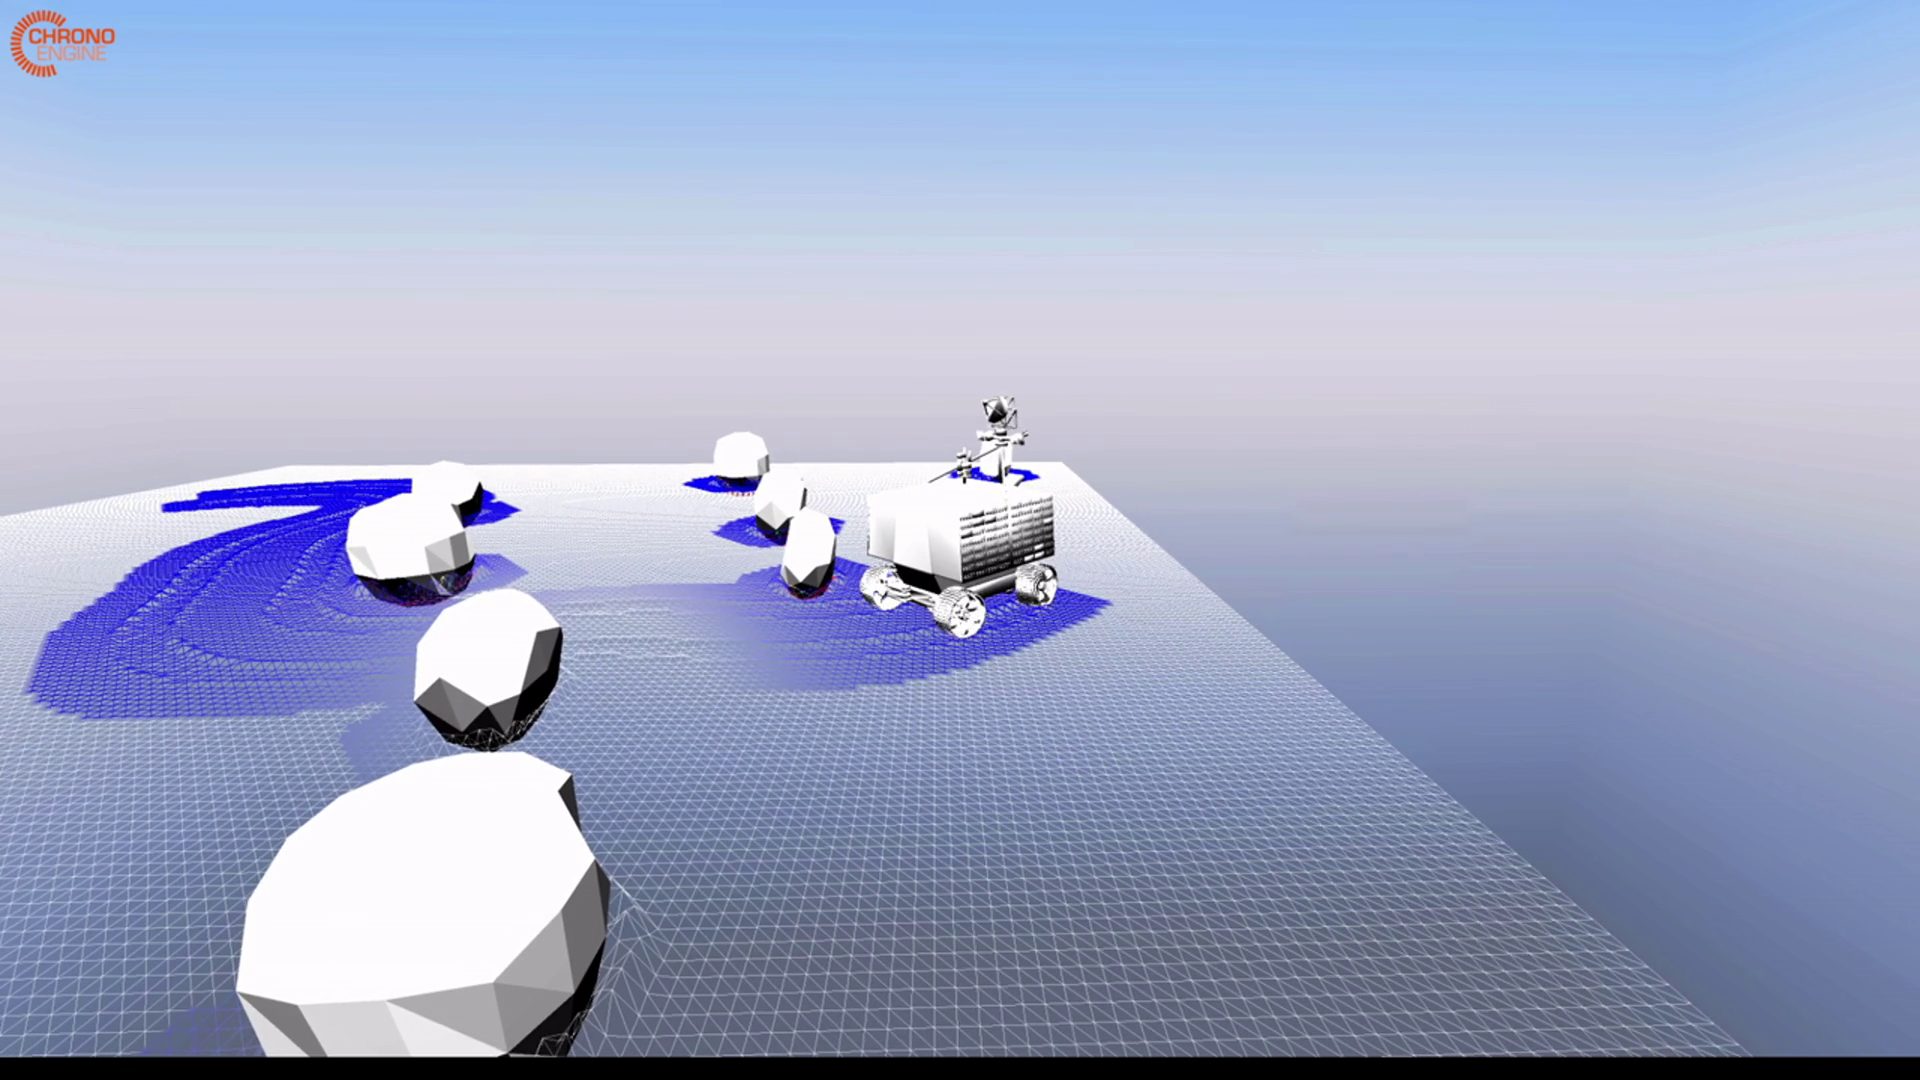
\includegraphics[width=0.45\textwidth]{Images/screenshot/3.png}}
	\subfigure[Scenario 4 \cite{sce-4}]{
		\label{fig:screen_4}
		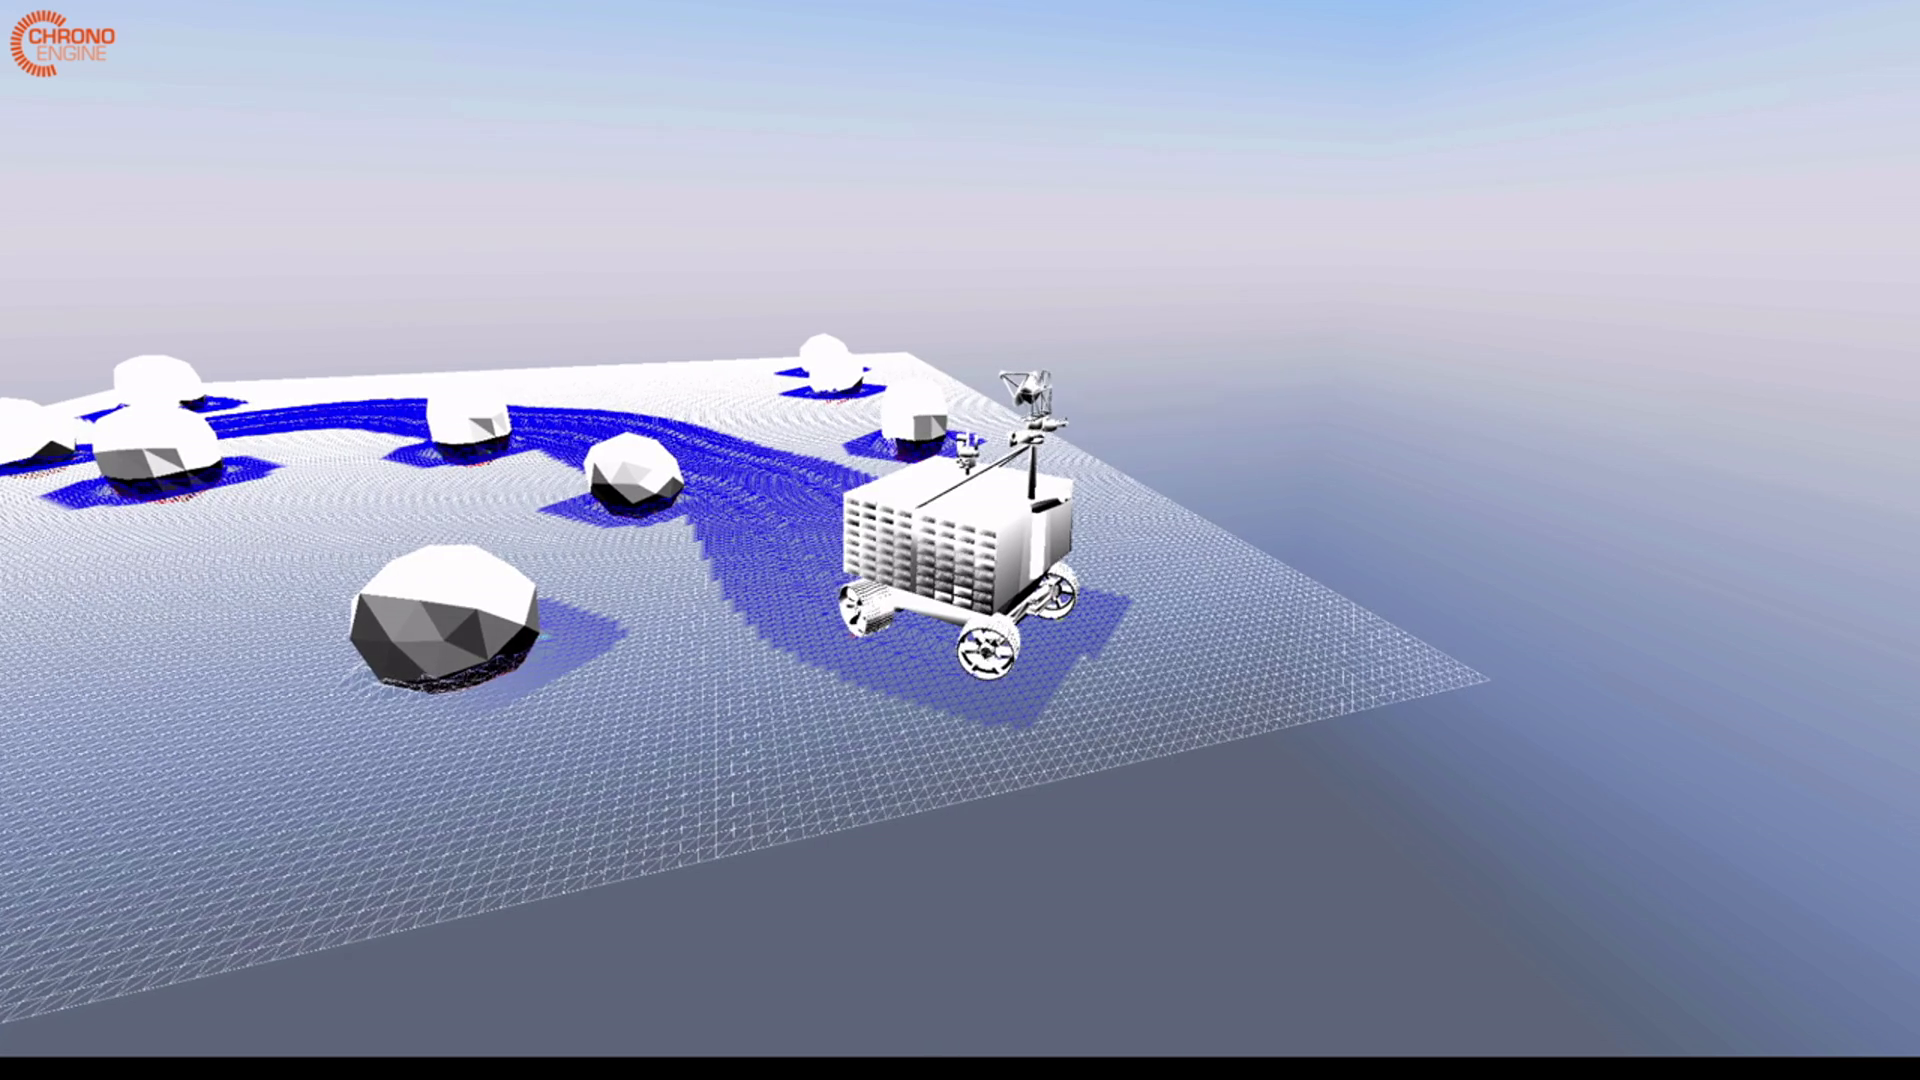
\includegraphics[width=0.45\textwidth]{Images/screenshot/4.png}}
	
	\caption{Screenshot of the simulation for each scenario. Full simulation animation can be found in the corresponding citation entry. }
\end{figure}

\begin{figure}
	\centering     %%% not \center
	\subfigure[Scenario 1]{
		\label{fig:traj_compare_1}
		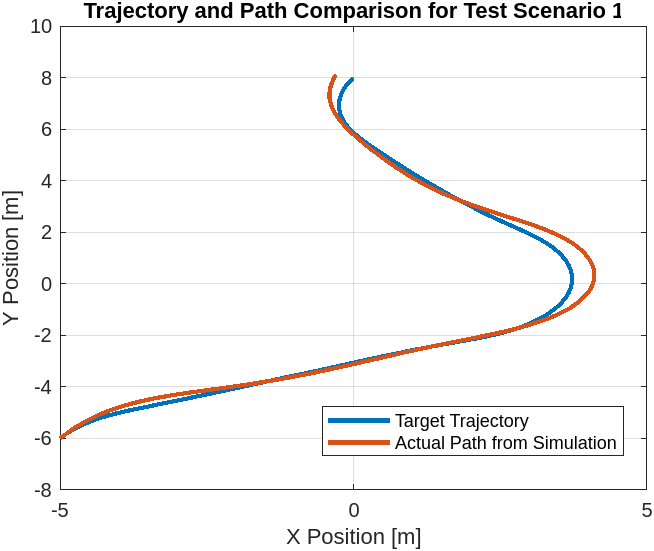
\includegraphics[width=0.45\textwidth]{Images/traj/1.png}}
	\subfigure[Scenario 2]{
		\label{fig:traj_compare_2}
		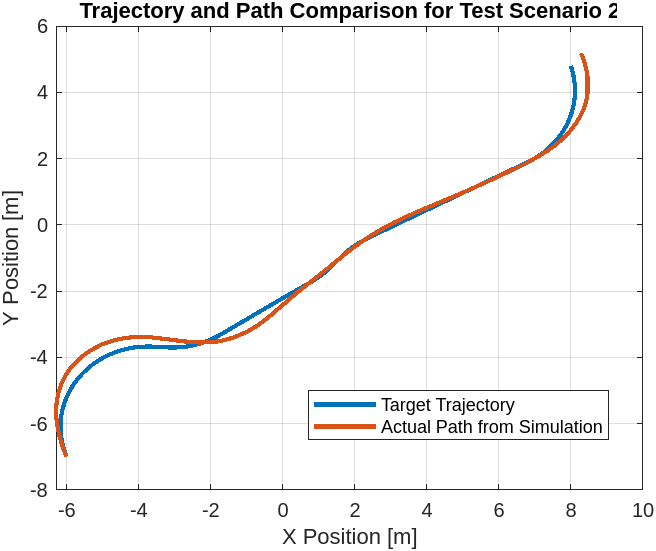
\includegraphics[width=0.45\textwidth]{Images/traj/2.png}}
	\subfigure[Scenario 3]{
		\label{fig:traj_compare_3}
		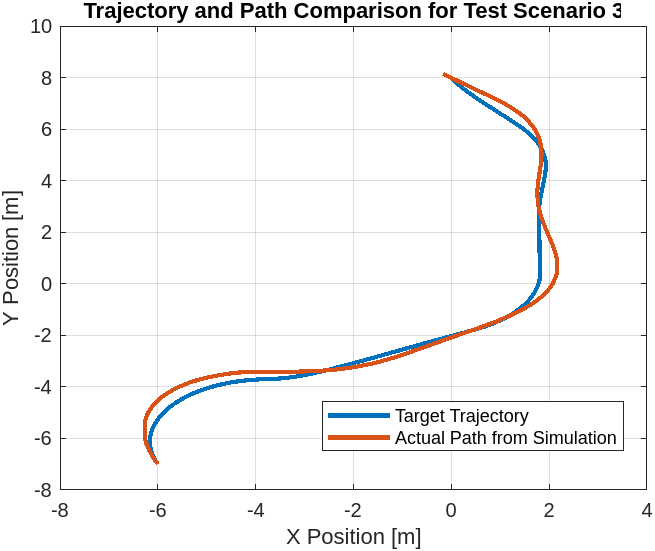
\includegraphics[width=0.45\textwidth]{Images/traj/3.png}}
	\subfigure[Scenario 4]{
		\label{fig:traj_compare_4}
		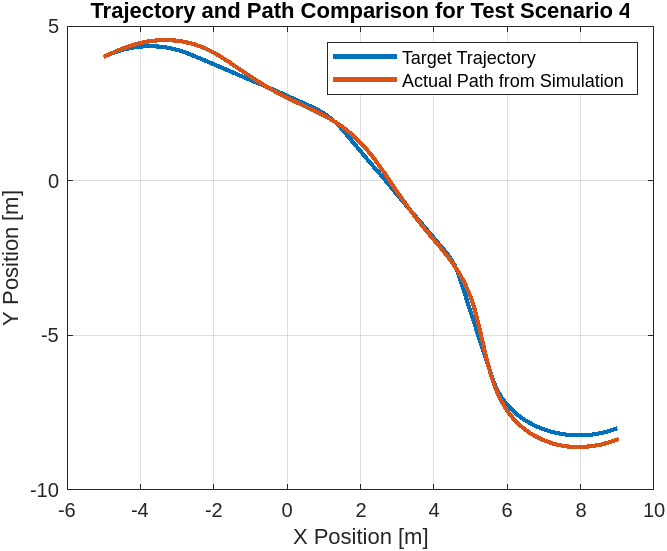
\includegraphics[width=0.45\textwidth]{Images/traj/4.png}}
	
	\caption{Comparison between target trajectory and the actual simulation path for each scenario. Note that the trajectory tracking in enforced by using a PID controller.}
\end{figure}

\begin{figure}
	\centering     %%% not \center
	\subfigure[Scenario 1]{
		\label{fig:data_1}
		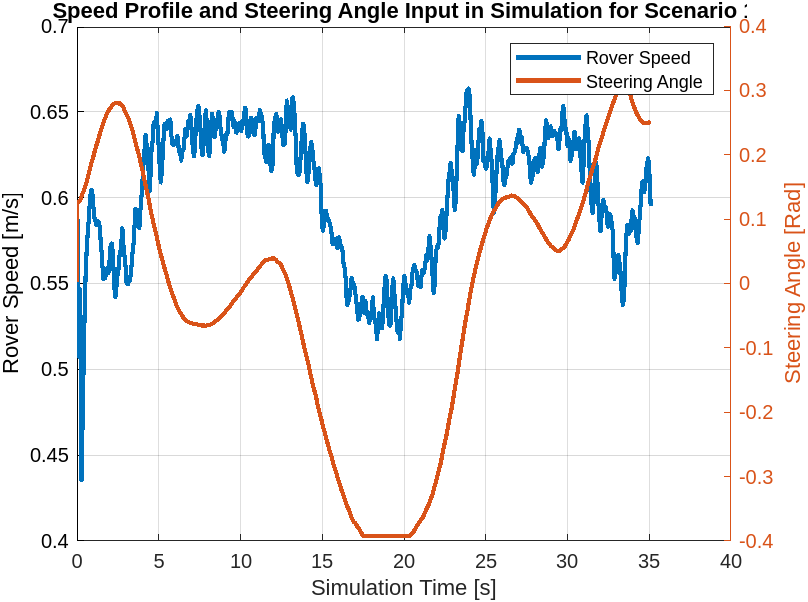
\includegraphics[width=0.45\textwidth]{Images/data/1.png}}
	\subfigure[Scenario 2]{
		\label{fig:data_2}
		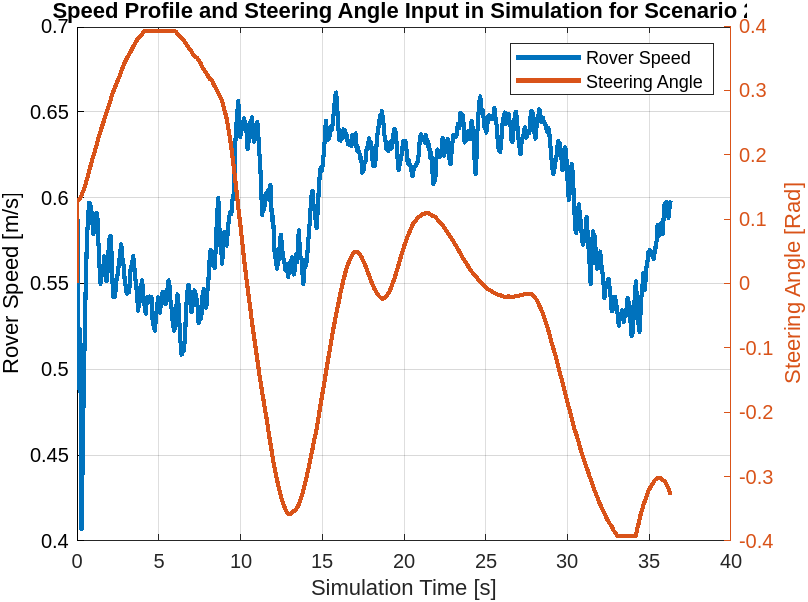
\includegraphics[width=0.45\textwidth]{Images/data/2.png}}
	\subfigure[Scenario 3]{
		\label{fig:data_3}
		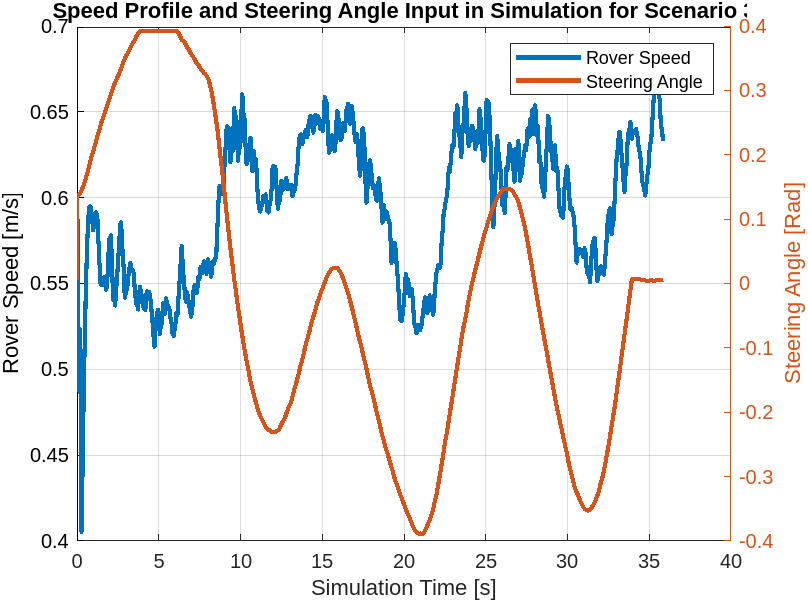
\includegraphics[width=0.45\textwidth]{Images/data/3.png}}
	\subfigure[Scenario 4]{
		\label{fig:data_4}
		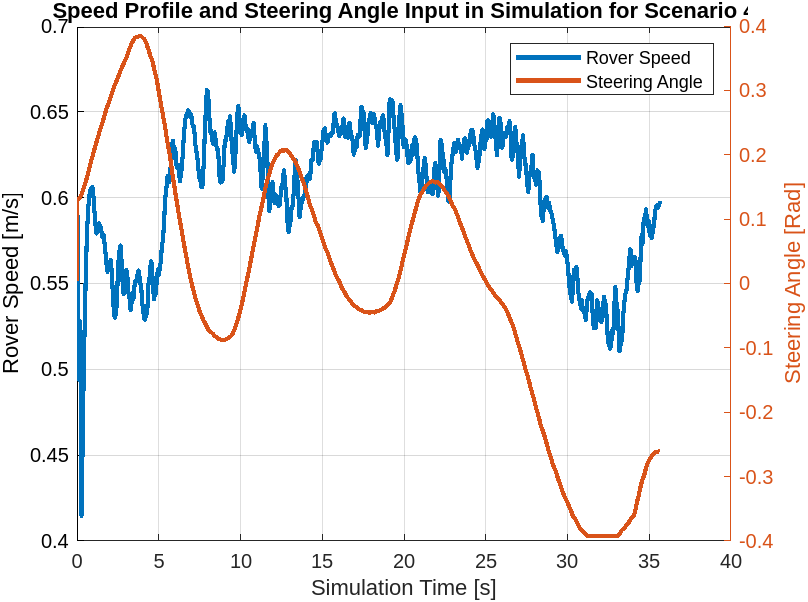
\includegraphics[width=0.45\textwidth]{Images/data/4.png}}
	
	\caption{Rover's speed profile and steering angle input in the simulation for each scenario. }
\end{figure}



\section{Limitation and Future Work}

We assume the control algorithm can obtain privileged information, such as the size of the terrain, the exact locations and the sizes of the obstacles, and the rover location due to the time limitation of the course project. However, we plan to extend the research focus to replicate what happens in real-life engineering - the environment, obstacles information, and rover information are all acquired through sensing, such as camera sensors, lidar sensors, radar sensors, and potentially position sensors. As Project Chrono can simulate sensor data, such as shown in Figure \ref{fig:curiosity_chrono}, in the near future, we will conduct research to reconstruct the 3d environment and obtain the terrain and obstacle data from the "real" environment. 

\bibliographystyle{ieeetr}
\bibliography{sample}

\end{document}